% !TEX root = ../manuscript.tex

%%%%%%%%%%%%%%%%%%%%%%%%%%%%%%%%%%%%%%%%%%%%%%%%%%%%%%%%%%%%%%%%%%%%%
%% Start the main manuscript here.
%%%%%%%%%%%%%%%%%%%%%%%%%%%%%%%%%%%%%%%%%%%%%%%%%%%%%%%%%%%%%%%%%%%%%

\section{Introduction}

Biogas capture from landfill sites or wastewater treatment plants is identified
as an appealing strategy to procure a renewable energy fuel, simultaneously
promoting a reduction in greenhouse gas emissions and an increase in waste
treatment profitability \citep{themelisMethaneGenerationLandfills2007}. The use
of biogas as an energy green resource critically calls for a substantial
increase of its \ce{CH4} quality by removing gaseous and vapour impurities
resulting from anaerobic digestion processes
\citep{themelisMethaneGenerationLandfills2007}. One prominent class of biogas
impurities are the linear (denoted ``L'') and cyclic (denoted ``D'') siloxanes,
as degradation by-products of silicone polymers from packaging, construction,
cosmetics, and household items
\citep{takuwaCharacterizationTraceConstituents2009,
ohannessianVolatileOrganicSilicon2008}. This family of molecules is also known
to damage subsequent energy recovery systems, e.g. combustion engines, fuel
cells and steam reformers, via their decomposition into amorphous silica on
heated surfaces that leads to abrasive solid deposits on critical machinery, and
to inactivation of gas reforming catalysts
\citep{wangRecentAdvancesTechnologies2019}. Octamethylcyclotetrasiloxane
commonly labelled D4 is the most representative siloxane species present in
biogas, which spans from 50 to 70\% of the total siloxane content due to its
relatively low water solubility (\SI{56}{\micro\gram\per\litre}) and its
significant vapour pressure (\SI{196}{\pascal} at \SI{303}{\kelvin})
\citep{ohannessianVolatileOrganicSilicon2008,
wangRecentAdvancesTechnologies2019, dewilEnergyUseBiogas2006}.

Multiple technologies have been proposed to mitigate the presence of siloxanes
in biogas outlet streams, including mineral acid/base scrubbing, deep chilling,
or iron oxide beds, often working in tandem to remove other impurities
\citep{kuhnRequirementsTechniquesCosts2017}. The physisorption-based removal of
D4 by porous filters is also a promising alternative, due to its relatively low
potential energetic cost, while avoiding the use of environmentally hazardous
chemicals \citep{chinStatisticalAnalysisTrace2020,
ajharSiloxaneRemovalLandfill2010}. A variety of conventional adsorbents has been
envisaged for siloxane elimination, including activated carbons
\citep{finocchioDecompositionHexamethylcyclotrisiloxaneSolid2008}, zeolites
\citep{montanariPurificationLandfillBiogases2010}, and silicas
\citep{sigotAdsorptionOctamethylcyclotetrasiloxaneD42015}. However, these
materials suffer from several drawbacks that limit their use, in particular
insufficient uptake and/or incomplete regeneration under standard conditions.
Moreover, downstream biogas commonly contains a proportion of water, which can
compete with D4 sorption when using hydrophilic adsorbents
\citep{kuhnRequirementsTechniquesCosts2017,schweigkoflerRemovalSiloxanesBiogases2001}.
Therefore, finding a high capacity adsorbent capable of removing siloxanes under
moderate humidity conditions in a reversible manner remains a challenge.

\begin{widefigure}[htb]
    \centering
    \includegraphics[width=0.95\textwidth]{ensemble_schema}
    \caption{%
        Workflow of the strategy applied to identify the best MOFs for
        D4 adsorption, narrowing down candidates from top to bottom through
        synergistic computational (left) and experimental (right) actions. The
        final MOF candidate, PCN-777, is highlighted.
    }\label{fig:overview}
\end{widefigure}

Metal-Organic Frameworks (MOFs) are one of the most recent classes of porous
adsorbents. These coordination polymers are built from the assembly of metal
nodes and organic multidentate linkers to form architectures of different
dimensionality from 1D to 4D \citep{fereyHybridPorousSolids2008,
zhouIntroductionMetalOrganic2012,
evansFourdimensionalMetalorganicFrameworks2020}. Their near-infinite diversity,
thanks to a wide set of building blocks, has made this class of porous solids
promising for applications in gas/vapour adsorption/separation
\citep{siegelmanChallengesOpportunitiesAdsorptionbased2019,
linMicroporousMetalOrganicFramework2020}, catalysis
\citep{bavykinaMetalOrganicFrameworks2020}, and sensing
\citep{allendorfElectronicDevicesUsing2020,
woellnerAdsorptionDetectionHazardous2018} among others. Their high and uniform
porosity combined with extensive chemical tunability of their pore walls suggest
that MOFs may hold promise as candidates for siloxane adsorption. Insofar only
two studies have attempted to investigate the potential of MOFs for D4 removal.
Mito-Oka and co-workers \citep{mito-okaSiloxaneD4Capture2013} proposed DUT-4(Al)
(\ce{[Al(OH)(2,6-ndc)}, DUT: Dresden University of Technology), a wine rack-like
MOF, as a first potential adsorbent. Although its hydrophobicity makes this MOF
attractive for D4 elimination under humidity, its adsorption capacity of
\SI{0.15}{\gram\per\gram}, estimated through single component by TGA
measurements, is rather low and its regeneration can only be achieved at very
high temperature, over \SI{523}{\kelvin}, resulting from a high confinement of
D4 (kinetic diameter of \SI{8.6}{\angstrom}) in its channels (9 Å × 9 Å). More
recently, MIL-101(Cr) (\ce{Cr3O(OH)(H2O)2(btc)3}, MIL: Material of Institute
Lavoisier), a well-known highly porous MOF incorporating two types of mesoporous
cages with diameters of 29 Å and 34 Å was demonstrated to exhibit a much higher
D4 uptake of \SI{0.95}{\gram\per\gram} at \SI{298}{\kelvin}, however its
regeneration was only possible upon heating at \SI{423}{\kelvin} under vacuum
\citep{gargiuloChromiumbasedMIL101Metal2019}. Further, since MIL-101(Cr) is
known to be highly hydrophilic \citep{zhaoSynthesisMIL101Cr2020} we can expect a
substantial drop of its D4 uptake performance even under low-relative humidity.
Indeed, neither of these MOFs tested so far combines a large D4 uptake,
low-energy regeneration and hydrophobicity to avoid a preferential adsorption of
\ce{H2O} over D4 under low to moderate relative humidity.

To date, only a very small number of MOFs has been sampled for this application,
and therefore relied on researchers' intuition to identify promising adsorbents.
There are, however, a myriad of hydrophobic MOFs that might perform better for
D4 adsorption. Since it is unfeasible to individually test the performances of
all the existing MOFs, several high throughput computational screening (HTCS)
workflows have been devised which identified promising MOFs for diverse
adsorption-related applications \citep{simonWhatAreBest2015,
parkEstablishingUpperBounds2017, moghadamComputeraidedDiscoveryMetal2018,
boydDatadrivenDesignMetal2019, shiMachineLearningSilico2020,
yaoInverseDesignNanoporous2021}. However, such a computational strategy can only
be successful if conducted in strong interplay with a careful analysis of the
best-predicted MOF performers in terms of chemical/thermal stability under the
target working conditions as well as ease of synthesis/activation. This enables
the selection of the MOF candidate with the best overall compromise for further
adsorption testing to confirm the expectation.

With this in mind, we herein devise a hand-in-hand computational-experimental
strategy whose workflow is summarized in \cref{fig:overview}. As a first stage,
the CoRE (Computation-Ready, Experimental) MOF 2019 database
\citep{chungAdvancesUpdatesAnalytics2019} was computationally screened with the
objective to identify hydrophobic materials showing a D4 uptake higher than the
current MOF benchmark, e.g. MIL-101(Cr). Notably, the microscopic models used to
describe both MOF and D4 were validated by a good agreement between the
simulated D4 uptake and our own experimental data collected on the two MOFs
mentioned above, i.e. MIL-101(Cr) and DUT-4 (Al). From the top 56 predicted MOF
performers, we selected the Zr carboxylate-based mesoporous PCN-777 (PCN for
Porous Coordination Network) for further experimental testing. This MOF was
demonstrated to exhibit not only a record D4 uptake (\SI{1.8}{\gram\per\gram})
to date for a crystalline porous material, but also exceptional cycling and
low-energy regeneration without the need for thermal treatment, while its
confirmed hydrophobicity strongly suggests a preservation of its adsorption
performance under low to moderate relative humidity conditions. An in-depth
analysis of the adsorption mechanism further revealed the dominant host-guest
interactions that control the adsorption of the first D4 molecules and their
effective packing in the whole porosity up to saturation.

\section{Methodology}\label{methodology}

\subsection{Computational methods}\label{methodology-computational}

We used the CoRE-MOF 2019 database \citep{chungAdvancesUpdatesAnalytics2019}
(over 14 000 MOFs), recently updated to remove solvent molecules and disordered
structures, to which we also added further 29 well-known MOFs owing to their
good chemical/thermal stability and permanent accessible porosity (listed in
\cref{tbl:extra-mofs} SI). The geometric characterization of MOFs, including
pore limiting diameters (PLDs), densities, \ce{N2}-accessible surface areas
(SAs), pore volumes (PVs) and void fractions (\(\phi\)), were calculated by
Zeo++ software \citep{willemsAlgorithmsToolsHighthroughput2012}. All Monte Carlo
simulations were performed with the RASPA simulation package
\citep{dubbeldamRASPAMolecularSimulation2016}. Henry coefficients of \ce{H2O}
(\(K_{H,H_{2}O}\)) and isosteric enthalpy of adsorption (\(\Delta
H_{st,H_{2}O}^{0}\)) were initially computed at \SI{298}{\kelvin} for all MOFs
using the Widom particle insertion method
\citep{frenkelUnderstandingMolecularSimulation2002}. These simulations were
carried out using 1 × 10\textsuperscript{5} production cycles and 5 ×
10\textsuperscript{4} cycles for equilibration. We applied the same Widom
insertion method to calculate isosteric enthalpy of adsorption at low coverage
for D4 in DUT-4(Al) and PCN-777 with the consideration of 1 × 10\textsuperscript{6}
production cycles and 5 × 10\textsuperscript{5} steps for equilibration.
Continuous fractional component Monte Carlo (CFCMC) simulations
\citep{rahbariRecentAdvancesContinuous2020} were performed to evaluate the
saturation D4 uptake of all the selected hydrophobic MOFs at \SI{298}{\kelvin}.
All CFCMC simulations were carried out for a total of 1 × 10\textsuperscript{4}
cycles with 5 × 10\textsuperscript{3} cycles for equilibration. A cycle consists
of N Monte Carlo steps, where N is equal to the number of molecules (which
fluctuates during a CFCMC simulation). For each cycle, random insertion,
rotation, translation and continuous-fractional swap moves were attempted. The
D4/MOF and \ce{H2O}/MOF interactions were described by the sum of van der Waals
(Lennard-Jones) and Coulombic terms. The electrostatic interactions were
calculated by the Ewald summation \citep{ewaldBerechnungOptischerUnd1921} while
a cut-off radius of 12.8 Å was considered for the van der Waals term. Indeed,
unit cell dimensions were increased to at least 25.6 Å in each three directions
for all MOFs and their frameworks were treated as rigid. Atomic charges for all
atoms in the MOFs were estimated using Extended Charge Equilibration (Qeq)
method as implemented in RASPA \citep{dubbeldamRASPAMolecularSimulation2016} and
their LJ parameters were taken from the UFF forcefield as currently employed
\citep{qiaoHighthroughputComputationalScreening2017,
keskinProgressOpportunitiesChallenges2009}. H2O was modelled using TIP4P/2005
\citep{abascalGeneralPurposeModel2005}. D4 was described by a semi-flexible all
atom model with intramolecular parameters taken from the consistent-valence
force field (CVFF) \citep{dauber-osguthorpeStructureEnergeticsLigand1988}
(\cref{tbl:ff-d4-bond,tbl:ff-d4-bend,tbl:ff-d4-dihedral,tbl:ff-d4-cross-bond,tbl:ff-d4-cross-bondbend},
SI) while the LJ parameters for all atoms were taken from the UFF forcefield as
done in earlier work \citep{xuSolvationForceSimulations2014} and their charges
were calculated at the DFT level (\cref{tbl:ff-d4-charge}, SI).

All the results of the HCTS are available as CSV files in the SI. A web-based
explorer, which can be used to interactively display the dataset is available at
\url{https://pauliacomi.com/mof4d4}.

\subsection{MOF sorbents}\label{methodology-benchmark}

The benchmark MIL-101(Cr) sample was taken from a previous work
\citep{pillaiCapturePerformancesHybrid2017}, with all textural characteristics
as stated in reference. DUT-4(Al) was purchased from Materials Center (TU Dresden,
Germany). PXRD, TGA and \ce{N2} physisorption measurements for DUT-4(Al) are
available in the SI (\cref{fig:dut4-summary}). Brunauer-Emmet-Teller (BET) areas
of \SI{3475}{\metre\squared\per\gram} and \SI{1610}{\metre\squared\per\gram}
were determined for MIL-101(Cr) and DUT-4(Al), respectively. PCN-777 was synthesised
by optimizing a previous published methodology
\citep{fengHighlyStableZeotype2015}. Full synthesis methodology, activation
procedure and phase purity analysis using TGA, PXRD and \ce{N2} physisorption
are given in the SI. All samples were activated at \SI{423}{\kelvin} under
vacuum prior to adsorption experiments.

\subsection{Material characterization}\label{methodology-characterization}

PXRD patterns were recorded on a Panalytical X'Pert PRO PXRD diffractometer with
a Cu \(K_{\alpha}\) radiation source, in a Bragg-Brentano reflection geometry,
using a spinning sample holder with a low-background silicon insert. \ce{N2}
isotherms at \SI{77}{\kelvin} were recorded in a Micromeritics Tristar
manometric analyser (displayed in \cref{fig:n2-phys}, SI). The BET areas were
calculated using the pyGAPS suite \citep{iacomiPyGAPSPythonbasedFramework2019},
with the application of the Rouquerol rules for isotherm region selection
yielding a minimum Pearson correlation coefficient of \(R=0.997\) (see
\cref{fig:n2-analysis} for resulting fitting).

\subsection{D4 sorption experiments}\label{methodology-d4sorption}

Sorption measurements were gravimetrically recorded using a dynamic method in a
DVS Vacuum instrument (Surface Measurement Systems, UK). In this setup, a
continuous adsorbate flow sourced from the headspace of a reservoir enters the
sample enclosure, passes the suspended sample pan, and is entrained by a vacuum
system. Pressure is controlled by a butterfly valve located before the outlet.
Uptake is monitored by a magnetically suspended balance, capable of measuring
mass changes at a resolution of \SI{0.1}{\micro\gram}. The entire apparatus is
kept in a temperature-controlled chamber to avoid any condensation points. For
each experiment, a stainless-steel sample pan is first tared, then loaded with
about \SI{10}{\milli\gram} of sample. The sample is activated \emph{in situ}
under dynamic vacuum (\SI{1E-2}{\pascal}) to \SI{423}{\kelvin}. The
adsorption-desorption isotherms for D4 and \ce{H2O} and subsequent repeats were
recorded at \SI{303}{\kelvin} in the 0-\SI{10}{\pascal} range of pressure.
Adsorption cycling was similarly recorded, switching between two setpoints of
low (\SI{0.5}{\pascal}) and high pressure (\SI{10}{\pascal}). The D4 used for
the sorption experiments was sourced from Sigma Aldrich, with minimum 98\%
purity.

\begin{widefigure}[b]
    \centering
    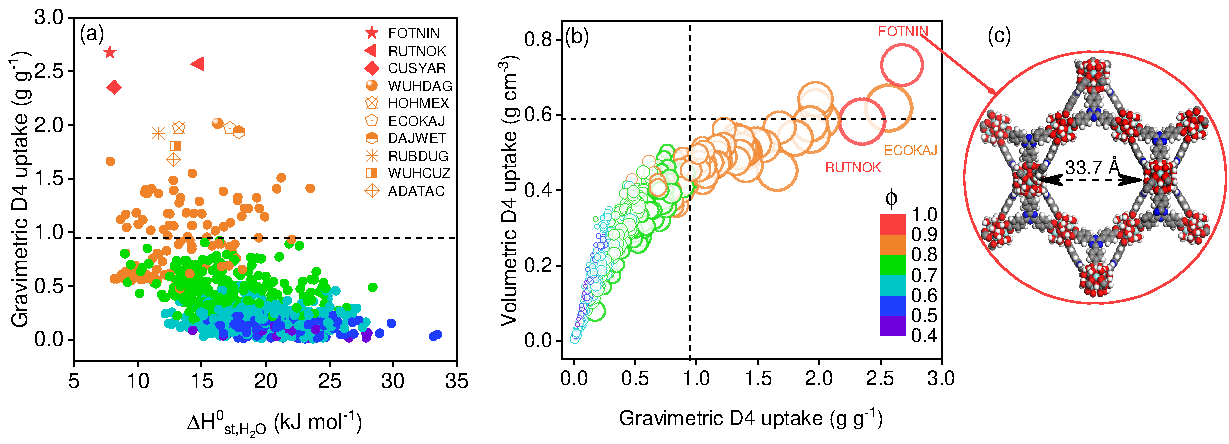
\includegraphics[width=0.9\textwidth]{screening}
    \caption{%
        (a) Predicted D4 uptake performance at \SI{298}{\kelvin} for the
        hydrophobic MOF database plotted as a function of computed \(\Delta
        H_{st,H_{2}O}^{0}\), and colour coded by void fraction, \(\phi\). Top
        performing 10 candidates are represented by different symbols in the
        legend. (b) Relation between gravimetric (\si{\gram\per\gram}) and
        volumetric (\si{\gram\per\centi\metre\cubed}) D4 uptake for all MOFs at
        \SI{298}{\kelvin}. Marker size represents PV while colour denotes
        \(\phi\). Dashed line represents the gravimetric and volumetric uptake
        of benchmark MIL-101(Cr)\citep{gargiuloChromiumbasedMIL101Metal2019}.
        (c) Illustration of the structure of our promising material identified for D4 uptake,
        PCN-777. Zr, N, O, C, and H atoms are depicted in light blue, dark blue,
        red, dark grey, and light grey, respectively.
    }\label{fig:d4-screening}
\end{widefigure}

\section{Results and discussion}\label{results-and-discussion}

\subsection{Pre-selection of hydrophobic MOFs}\label{pre-screening}

We first excluded from our considered MOF database all structures with PLDs
lower than 6 Å, a threshold selected as the average between the kinetic diameter
of D4 (8.6 Å) and the effective diameter of its constitutive inner Si-O ring
(4.5 Å). A total of 1739 remaining non-disordered MOFs were further considered,
their geometric and textural properties, i.e. PV, SA, and \(\phi\), as well as
their density (\(\rho\)) being summarized in \cref{fig:d4-screening-geometric}.
As siloxane-rich biogas streams often contain water vapour, the optimal D4
adsorbent should have a relatively low water affinity to avoid competing
adsorption. Moreover, hydrophobic MOFs are known to possess increased resistance
to the hydrolysis of the metal-linker bond
\citep{burtchWaterStabilityAdsorption2014,
wuEnhancingStabilityMetalorganic2010}, alleviating long-term water stability
concerns. Therefore, we screened the water affinity of the 1739 MOFs by
computing their Henry coefficient of water (\(K_{H,H_{2}O}\)) and the isosteric
enthalpy of adsorption at infinite dilution (\(\Delta H_{st,H_{2}O}^{0}\)) at
\SI{298}{\kelvin} using the Widom particle insertion method
\citep{frenkelUnderstandingMolecularSimulation2002}. This approach is generally
applied in HTCS studies, providing a quick way to gauge the
hydrophobicity/hydrophilicity of MOFs
\citep{matito-martosDiscoveryOptimalPorous2018,
qiaoHighthroughputComputationalScreening2017}. All the computational details
including the force fields used to describe both MOFs and water are provided in
the methodology section and SI. In the frame of biogas upgrading, an extremely
hydrophobic adsorbent is not required since the water content usually ranges
from 38\% to 85\% relative humidity \citep{wangRecentAdvancesTechnologies2019},
therefore the following thresholds were applied to select MOFs with moderate to
high hydrophobicity: \(K_{H,H_{2}O}\) < \SI{1e-5}{\mol\per\kilo\gram\per\pascal}
and \(\Delta H_{st,H_{2}O}^{0}\) < \SI{33}{\kilo\joule\per\mol} (below the
vaporization enthalpy of water \textasciitilde \SI{40}{\kilo\joule\per\mol})
\citep{lemmonNISTStandardReference2018}. As a frame of reference, the highly
hydrophobic ZIF-8 is characterized by \(K_{H,H_{2}O} =\)
\SI{2.5E-6}{\mol\per\kilo\gram\per\pascal} and \(\Delta H_{st,H_{2}O}^{0} = \)
\SI{30}{\kilo\joule\per\mol}
\citep{moghadamEfficientIdentificationHydrophobic2016}. Overall, among the 1739
MOFs, 811 structures (47\% of our material library) were predicted to fulfill
these two criteria. This hydrophobic MOF dataset encompasses structures of
density ranging from \SI{0.24}{\gram\per\centi\metre\cubed} to
\SI{2.04}{\gram\per\centi\metre\cubed} and with a wide range of geometric and
textural features: 6 Å < PLD < 36 Å, 0.42 < \(\phi\) < 0.90,
\SI{0.27}{\centi\metre\cubed\per\gram} < PV <
\SI{3.72}{\centi\metre\cubed\per\gram} and \SI{320}{\metre\squared\per\gram} <
SA < \SI{6700}{\metre\squared\per\gram}, as shown in
\cref{fig:d4-screening-geometric}.

\subsection{Prediction of the D4 uptake performance for the hydrophobic MOFs}\label{d4-screening}

\begin{widetable}[htb]
    \centering\small
    \caption{%
        Top 10 promising hydrophobic MOF materials identified for D4 uptake at \SI{298}{\kelvin}.
    }\label{tbl:top10}
    \begin{tabular}{@{}cccccccccc@{}}
        \toprule
        MOF & PLD & SA & \(\rho\) & PV & \(\phi\) & \(K_{H,H_{2}O}\) & \(\Delta H_{st,H_{2}O}^{0}\) &
        Gravimetric D4 & Volumetric D4 \\

        & (Å) & (\si{\metre\squared\per\gram}) & (\si{\gram\per\centi\metre\cubed}) & (\si{\centi\metre\cubed\per\gram}) & 
        & (\si{\mol\per\kilo\gram\per\pascal}) & (\si{\kilo\joule\per\mol}) & uptake (\si{\gram\per\gram}) & uptake (\si{\gram\per\centi\metre\cubed}) \\
        \midrule
        FOTNIN (PCN-777) & 28.36 & 2990 & 0.27 & 3.31 & 0.90 & \(2.80\times10^{-6}\) & 7.82 & 2.68 & 0.72\\
        RUTNOK & 14.65 & 6200 & 0.24 & 3.72 & 0.90 & \(6.70\times10^{-6}\) & 14.81 & 2.57 & 0.62\\
        CUSYAR & 12.18 & 5700 & 0.25 & 3.65 & 0.90 & \(3.42\times10^{-6}\) & 8.15 & 2.35 & 0.59\\
        WUHDAG & 10.50 & 5500 & 0.29 & 2.99 & 0.87 & \(4.69\times10^{-6}\) & 16.28 & 2.01 & 0.58\\
        HOHMEX & 14.89 & 5000 & 0.32 & 2.74 & 0.87 & \(4.66\times10^{-6}\) & 13.24 & 1.97 & 0.63\\
        ECOKAJ & 17.58 & 3600 & 0.33 & 2.68 & 0.87 & \(6.89\times10^{-6}\) & 17.20 & 1.97 & 0.65\\
        DAJWET & 26.59 & 5000 & 0.28 & 3.06 & 0.87 & \(7.73\times10^{-6}\) & 17.92 & 1.93 & 0.54\\
        RUBDUP & 19.25 & 4200 & 0.30 & 2.90 & 0.87 & \(3.79\times10^{-6}\) & 11.62 & 1.93 & 0.58\\
        WUHCUZ & 12.21 & 5500 & 0.30 & 2.91 & 0.87 & \(3.75\times10^{-6}\) & 12.94 & 1.80 & 0.54\\
        ADATAC & 10.28 & 5130 & 0.34 & 2.57 & 0.87 & \(4.16\times10^{-6}\) & 12.78 & 1.68 & 0.57\\
        \bottomrule
    \end{tabular}
\end{widetable}

As a validation stage of the computational method, the D4 uptakes for
MIL-101(Cr) and DUT-4(Al) were first predicted using the CFCMC approach described in
the methodology section and compared with the available experimental data. The
simulated uptake for MIL-101(Cr), the current best MOF performer, was found to
be \SI{1.03}{\gram\per\gram} vs. \SI{0.95}{\gram\per\gram} as reported in the
original experimental study \citep{gargiuloChromiumbasedMIL101Metal2019}. We
equally confirmed the good agreement between the calculated and the experimental
D4 uptake by recording an additional adsorption isotherm on a MIL-101(Cr)
sample, finding a D4 capacity of \SI{1.15}{\gram\per\gram} at \SI{298}{\kelvin}.
The D4 uptake for DUT-4(Al) was however predicted to be substantially higher
(\SI{0.42}{\gram\per\gram}) than the experimental value reported previously of
\SI{0.15}{\gram\per\gram} \citep{mito-okaSiloxaneD4Capture2013}. We therefore
collected a D4 adsorption isotherm on a pristine DUT-4(Al) sample, finding a D4
uptake of \SI{0.5}{\gram\per\gram} (\cref{fig:d4-benchmark}), more in line with
our theoretical assessment. The lower D4 capacity reported in the original study
is attributed to the method used to quantify the adsorbed amount, based on mass
loss upon heating. It is likely that only a fraction of D4 was released, since
D4 was demonstrated to strongly interact with DUT-4(Al) due to a high confinement in
its pores \citep{mito-okaSiloxaneD4Capture2013}.

Overall, the good agreement between the simulated uptakes and the corresponding
experimental data for the previously investigated MOFs served to validate both
the applicability of our computational method and the reliability of our
experimental setup. This further highlights the importance of a dual
experimental-computational approach even prior to starting the high-throughput
screening. We then transitioned towards the search for better performers amongst
the 811 identified hydrophobic MOFs. \cref{fig:d4-screening}a reports their
computed D4 uptakes vs. their \(\Delta H_{st,H_{2}O}^{0}\) values at
\SI{298}{\kelvin}, with a similar correlation depicted vs. \(K_{H,H_{2}O}\) in
\cref{fig:d4-screening-henryc}, SI. The dashed line represents the current known
upper bound for D4 uptake in MOFs, considering MIL-101(Cr) as the benchmark
sorbent (\SI{0.95}{\gram\per\gram})
\citep{gargiuloChromiumbasedMIL101Metal2019}. 56 hydrophobic MOFs were predicted
to be more attractive candidates than MIL-101(Cr) on the basis of gravimetric D4
uptake. Common geometric and textural features of these MOF candidates are void
fractions \(\phi\) larger than 0.81 and pore volumes (PV) higher than
\textasciitilde \SI{1.7}{\centi\metre\cubed\per\gram}. Typically, the relation
between gravimetric D4 uptake and PV is shown in
\cref{fig:d4-screening-grav-volum}.

The 10 best MOFs showing the highest D4 uptakes ranging from 1.68 to
\SI{2.68}{\gram\per\gram} are highlighted in \cref{fig:d4-screening}a by their
Cambridge Structural Database (CSD) \citep{allenCambridgeStructuralDatabase2002}
refcode and listed in \cref{tbl:top10}. Notably, all these identified candidates
were found to be highly hydrophobic with associated \(K_{H,H_{2}O}\) of about
\SI{5E-6}{\mol\per\kilo\gram\per\pascal} and their \(\Delta H_{st,H_{2}O}^{0}\)
ranging from 8 to \SI{18}{\kilo\joule\per\mol} which make these adsorbents also
potentially effective under moderate humidity conditions. \cref{tbl:top10} shows
that the highly hydrophobic FOTNIN is predicted to exhibit the highest saturated
D4 uptake (\SI{2.68}{\gram\per\gram}), in relation with its high PV
(\SI{3.31}{\centi\metre\cubed\per\gram}) and large mesoporous cages (33.7 Å ×
28.4 Å). Remarkably, this gravimetric D4 loading translates into a spectacular
improvement as compared to MIL-101(Cr)
\citep{gargiuloChromiumbasedMIL101Metal2019}. RUTNOK (common name IRMOF-76
\citep{oisakiMetalOrganicFramework2010}) gave almost a similar D4 uptake
(\SI{2.57}{\gram\per\gram}) as FOTNIN, in part due to similar PV
(\SI{3.72}{\centi\metre\cubed\per\gram}) and \(\phi\) (0.9). Other candidates
exhibit high D4 uptakes, including CUSYAR (also known as MOF-210
\citep{furukawaUltrahighPorosityMetalOrganic2010}), WUHDAG and WUHCUZ (NU-1104,
and NU-1103 \citep{wangUltrahighSurfaceArea2015}, respectively). Full structural
properties of these 10 MOFs including organic ligands and metal sites are given
in \cref{tbl:top-mofs-detail}.

In the scope of the practical application of a sorbent for a filter bed or
column, volumetric uptake is a reliable metric due to its direct relation to
equipment sizing. Trade-offs between gravimetric and volumetric uptakes have
been previously reported for the storage of various fluids using porous
materials \citep{moghadamComputeraidedDiscoveryMetal2018}.
\cref{fig:d4-screening}b shows the relation between the computed gravimetric and
volumetric D4 uptakes for the hydrophobic MOFs database. Unlike gravimetric
uptake which increases indefinitely, the volumetric uptake in porous materials
is limited by the density of the adsorbate fluid phase, to which it
asymptotically approaches as framework density decreases (and void fraction
increases) \citep{bobbittHighthroughputScreeningMetal2016}. Interestingly FOTNIN
remains the top MOF performer in terms of volumetric uptake as well
(\SI{0.72}{\gram\per\centi\metre\cubed}, see \cref{fig:d4-screening}b). This MOF
(common name PCN-777 \citep{fengHighlyStableZeotype2015}) is built from large
planar tritopic linkers (4,4',4'\,'-s-triazine-2,4,6-triyl-tri-benzoate or TATB)
coordinated to \ce{Zr6}-oxoclusters in an antiprismatic fashion, forming
vertex-sharing supertetrahedra surrounding a mesoporous cage of 33.7 Å as
depicted in \cref{fig:d4-screening}c. These cages are interconnected by
hexagonal windows (30 Å) and are typically decorated by \ce{OH/H2O} moieties
coordinated to the remaining axial positions of the \ce{Zr6} node.

\subsection{Experimental assessment of the D4 sorption performance for the top MOF}\label{assessment}

\begin{widefigure}[htb]
    \centering
    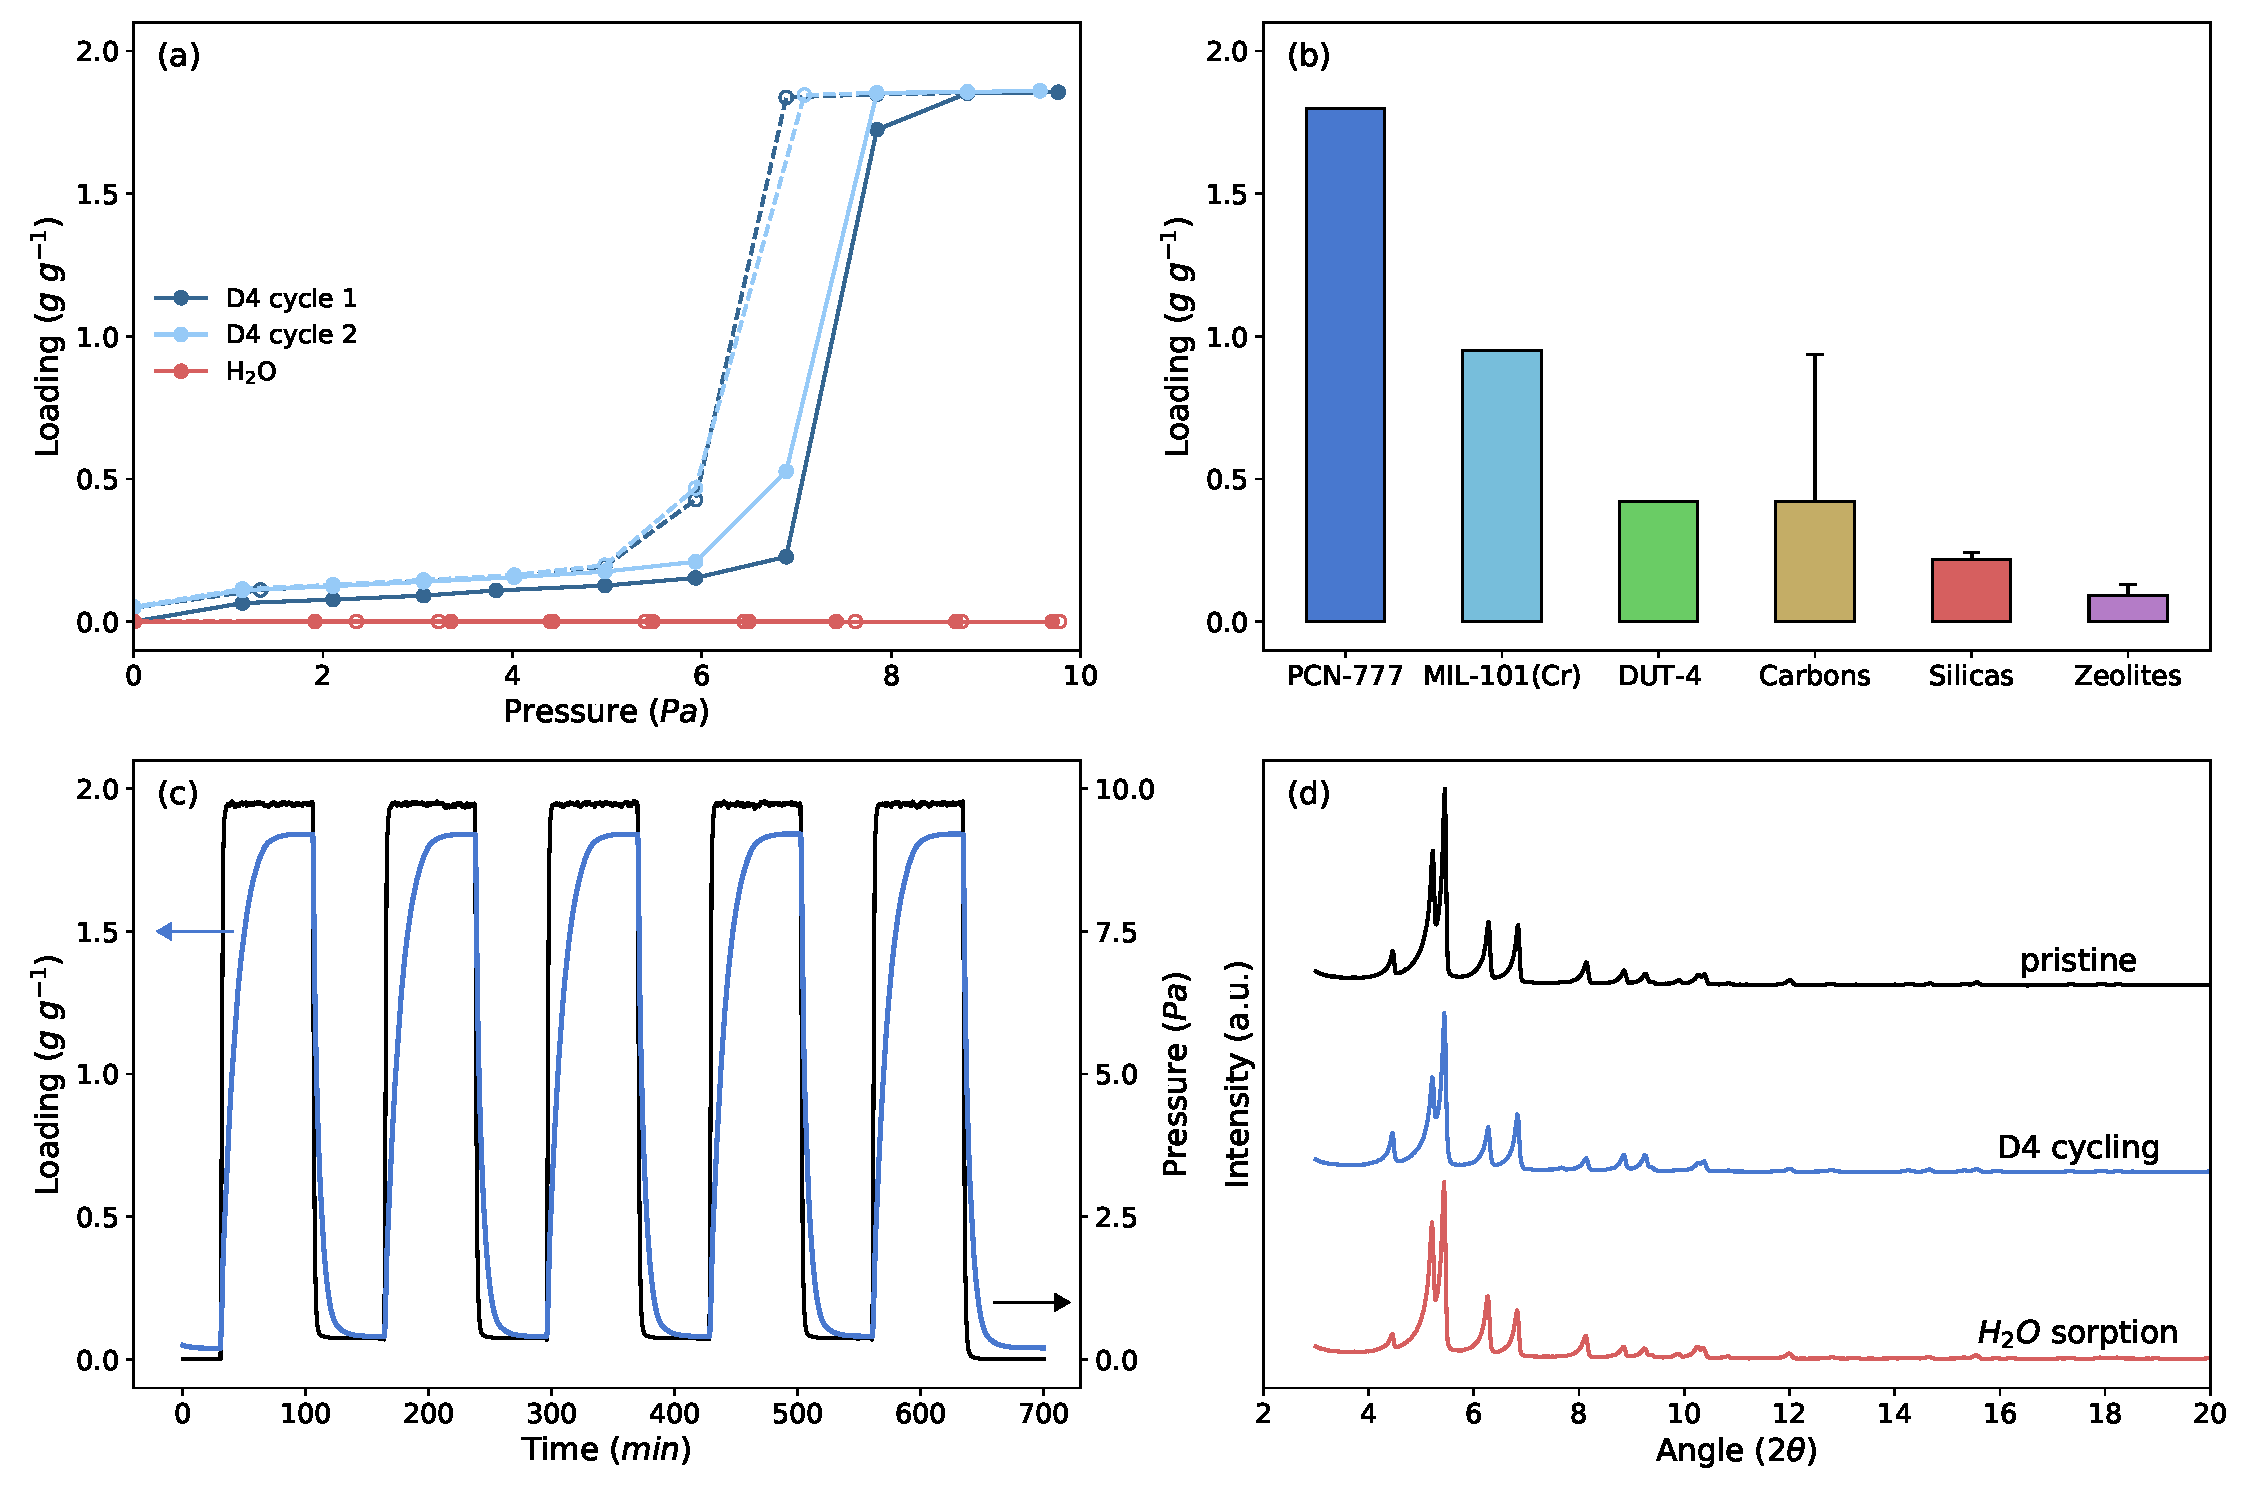
\includegraphics[width=0.95\textwidth]{d4-experiment}
    \caption{%
        (a) Single component adsorption/desorption isotherms for D4 (blue) and
        \ce{H2O} (red) collected at \SI{303}{\kelvin} for PCN-777 in the
        pressure range of 0-\SI{10}{\pascal} (corresponding to 0--0.05
        p/p\textsuperscript{0} for D4). Solid and open symbols represent
        adsorption and desorption branches, respectively. (b) Comparison of the
        D4 capacity of MOFs investigated in the present study with other classes
        of porous materials (data from
        \citet{wangRecentAdvancesTechnologies2019}), with error bars placed at
        one standard deviation of mean capacity. (c) 5 D4 sorption-desorption
        cycles recorded after the first two isotherms on PCN-777, in the same
        pressure range. (d) PXRD of pristine PCN-777 sample (black) and samples
        recovered after D4 cycling (blue) and water adsorption (red).
    }\label{fig:d4-experiment}
\end{widefigure}

While HTCS enabled a rapid and effective screening on the performance indicator,
additional criteria, such as thermal/chemical stability, synthesis route,
activation conditions, precursor toxicity and linker availability need to be
considered to select the optimal adsorbents. We therefore critically assessed
PCN-777 prior to further experimental action. Our selection criteria for PCN-777
were (i) the excellent known stability of the oxo-Zr-carboxylate metal node, at
the origin of the high chemical and thermal resistance of the framework,
alongside with (ii) the commercially available linker and well-controlled
synthesis procedure documented elsewhere \citep{fengHighlyStableZeotype2015,
liuPhotocatalyticHydrogenProduction2018}. Indeed, this material was synthesised
accordingly (details provided in the methodology section).

The D4 adsorption isotherm for PCN-777 was first recorded up to \SI{10}{\pascal}
at \SI{303}{\kelvin} using a dynamic vapour sorption system (experimental
details in the methodology section). The resulting isotherm, depicted in
\cref{fig:d4-experiment}a, exhibits a characteristic type V shape
\citep{thommesPhysisorptionGasesSpecial2015} with a sharp D4 uptake increase
above \SI{7}{\pascal} up to a maximum of \SI{1.8}{\gram\per\gram} that
translates into \SI{0.49}{\gram\per\centi\metre\cubed}. This value is however
lower than the predicted uptake due to two combined reasons: (i) an incomplete
evacuation of the porosity (theoretical PV=\SI{3.3}{\centi\metre\cubed\per\gram}
vs the experimental one of \SI{2.2}{\centi\metre\cubed\per\gram} determined
through \ce{N2} physisorption at \SI{77}{\kelvin}, in \cref{fig:n2-phys}, SI)
commonly observed for mesoporous MOFs
\citep{nelsonSupercriticalProcessingRoute2009, parkCrystalStructureGuest2007}
and (ii) only a partial accessibility of the super-tetrahedral cages to D4 owing
to their relatively small windows. Indeed, while optimized activation procedures
may recover more of the expected porosity, the attained D4 uptake constitutes a
record among porous solids. This positions PCN-777 as the crystalline porous
material with the highest currently known D4 uptake, almost twice higher than
the benchmark MIL-101(Cr), 5--10 times that of the most promising silicas and
zeolites, and above the best performing activated carbons as illustrated in
\cref{fig:d4-experiment}b \citep{wangRecentAdvancesTechnologies2019}. Notably,
the step-like adsorption behaviour is ideal from the application point of view
of a breakthrough filter, as it ensures a narrow mass transfer zone and
minimises the column dead zone at break point. Remarkably, the maximum uptake
for PCN-777 is attained at low pressure of \SI{7}{\pascal} that makes this MOF
highly promising for D4 removal in a gas phase concentration below 75 ppm.

\begin{widefigure}[htb]
    \centering
    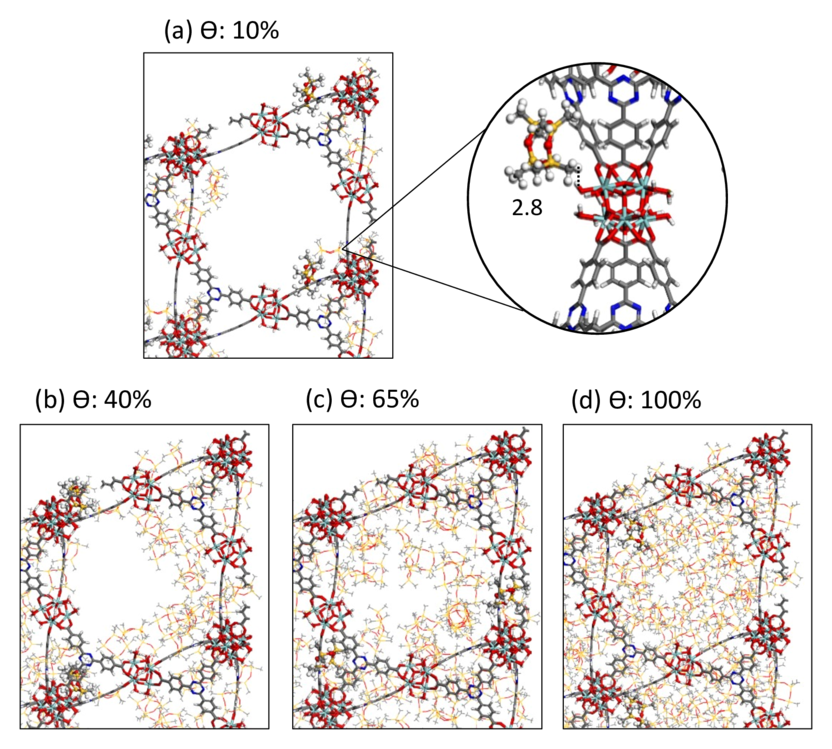
\includegraphics[width=0.7\textwidth]{mechanistic}
    \caption{%
        Representative snapshots of the preferential sitting of D4 in the pores
        of PCN-777 at \SI{298}{\kelvin} for increasing loading at (a) 10\% with
        highlighted interactions distance between D4 and the MOF framework, and
        at (b) 40\%, (c) 65\%, and (d) 100\% fractional loading (\(\theta\)).
        Framework atoms (sticks) and D4 molecules (lines, and ball and sticks)
        are coded as Zr, N, O, Si, C, and H atoms in light blue, dark blue, red,
        yellow, dark grey, and light grey respectively. The separating distance
        is represented by dashed black lines and reported in Å.
    }\label{fig:d4-mechanistic}
\end{widefigure}

Throughout desorption (dotted line with open symbols in
\cref{fig:d4-experiment}a), a small hysteresis occurs with a width of about
\SI{1}{\pascal}. Under complete vacuum, a minute amount of D4, about
\SI{0.1}{\gram\per\gram}, i.e. 5\% of total capacity, is retained in the
structure. We attribute this capacity loss to D4 molecules irreversibly trapped
in the super-tetrahedral cages or on a small fraction of defect sites. Overall,
PCN-777 acts as a highly reversible D4-adsorbent. A second sorption cycle
reveals the excellent repeatability of D4 sorption by this MOF, with identical
condensation pressure and total uptake, the adsorption-desorption branches now
overlapping in the very low-pressure region (\cref{fig:d4-experiment}a).

To further investigate the D4 adsorption-desorption cyclability of PCN-777, a
subsequent set of five cycles was recorded on the same sample, covering the
entire uptake range from fully loaded to empty under a medium vacuum level of
\SI{0.5}{\pascal} (see \cref{fig:d4-experiment}c). No further capacity loss is
observed after the initial 5 wt\% from cycle 1 to cycle 2 with a pressure drop
sufficient to fully remove adsorbed D4 in every cycle without the need of
thermal treatment. This is a leap forward compared to the previous MOF
candidates, i.e. MIL-101(Cr) and DUT-4(Al). The former was reported
\citep{gargiuloChromiumbasedMIL101Metal2019} to be fully regenerable only at
high temperatures (outgassed under vacuum at \SI{423}{\kelvin}), and we note
that vacuum alone was unable to fully desorb D4, with nearly 50\% of siloxane
remaining in the structure after desorption in our experiments
(\cref{fig:d4-benchmark}, SI). D4 adsorption in DUT-4(Al) is even more irreversible,
owing to the strong confinement of the siloxane molecules in its pores
\citep{mito-okaSiloxaneD4Capture2013}, with essentially no desorption observed
under vacuum (\cref{fig:d4-benchmark}, SI). The global sorption kinetics was
further qualitatively evaluated by observing the equilibration time throughout
cycling steps. \cref{fig:d4-experiment}c reveals that an adsorption/desorption
cycle can be achieved in less than 30 minutes. Such a fast kinetics is a clear
advantage for practical use. In addition, the water adsorption collected for
PCN-777 further confirmed its predicted hydrophobicity and revealed that below
\(P=\) \SI{7}{\pascal}, water loading is negligible, i.e. under
\SI{0.02}{\gram\per\gram} (see \cref{fig:d4-experiment}a). This observation
strongly suggests that PCN-777 is expected to maintain its high-level
performance for D4 removal under low to moderate humidity working conditions.

Stability of PCN-777 after its use as a D4 adsorbent was also evaluated by
checking its crystallinity and porosity. PXRD patterns recorded after the D4
cycling experiments show similar Bragg peak positions and broadenings as the
pristine material, testifying that no amorphisation or decrease of crystallinity
were incurred (\cref{fig:d4-experiment}d). The same conclusion holds true for
PCN-777 upon water adsorption. Further, \ce{N2} adsorption isotherms collected
at \SI{77}{\kelvin} for PCN-777 after \ce{H2O} and D4 adsorption both present a
similar shape than that of the pristine solid (see \cref{fig:n2-phys}). Slightly
lower pore volume (\SI{1.87}{\centi\metre\cubed\per\gram} vs
\SI{2.20}{\centi\metre\cubed\per\gram}) and BET area
(\SI{1544}{\metre\squared\per\gram} vs \SI{1730}{\metre\squared\per\gram}) were
obtained for the material after D4 cycling compared to the pristine solid,
attributed to the small amount of D4 retained in the porous framework during the
first adsorption cycle.

\subsection{Adsorption mechanism}\label{adsorption-mechanism}

A careful analysis of the adsorption mechanism of D4 in PCN-777 was further
explored by considering MC simulations in the canonical ensemble with increasing
loading up to the saturation. At the initial stage of adsorption, the
coordinated OH/\ce{H2O} moieties of the MOF \ce{Zr6} node pointing towards the
pore were found to act as primary adsorption sites (\cref{fig:d4-mechanistic}a).
The D4 molecule interacts mostly via its methyl group with an averaged
separating \ce{H(CH3)-H(H2O)} distance of 2.8 Å (see the radial distribution
function plotted for the corresponding pair in \cref{fig:d4-rdf}a) as
illustrated in \cref{fig:d4-mechanistic}a. This preferential sitting of D4 is
associated with a moderately high simulated adsorption enthalpy of
\SI{83.5}{\kilo\joule\per\mol} in line with the isosteric heat of adsorption we
assessed experimentally that ranges from 65 and \SI{75}{\kilo\joule\per\mol}
(\cref{fig:isosteric-enth}). Both values are higher than the enthalpy of
liquefaction of D4 at \SI{303}{\kelvin} as \SI{54.5}{\kilo\joule\per\mol}
\citep{lemmonNISTStandardReference2018}. We further demonstrated that this value
remains substantially lower than the one simulated for DUT-4(Al)
(\SI{194.0}{\kilo\joule\per\mol}) for which the adsorption of D4 is governed by
a high degree of confinement leading to an irreversible process. This
observation clearly states that the adsorption energetics in PCN-777 offers a
good compromise to ensure an efficient adsorption of D4 as well as an almost
fully reversible and fast adsorption/desorption process. While increasing the
loading, D4 molecules tend to form a monolayer near the wall of the cage owing
to their interactions with both the organic linkers and inorganic nodes of the
MOF as shown in \cref{fig:d4-mechanistic}b-c. Finally, at higher loading, the
molecules form multilayers and further occupy the whole cage corresponding to
the scenario of the capillary condensation (\cref{fig:d4-mechanistic}d). This
effective packing is governed by guest-guest interactions involving averaged
separating \ce{H(CH3)-H(CH3)} distance of 2.7 Å at saturation (the radial
distribution function plotted for this pair is shown in \cref{fig:d4-rdf}b).
Such pore filling mechanism has been commonly observed in diverse mesoporous
materials for a range of molecules \citep{rouquerolAdsorptionPowdersPorous2013}.
Indeed, PCN-777 exhibits an ideal combination of a large cage to enable an
effective packing of the siloxane molecules and the presence of moieties
accessible to D4 to favour moderately high host/guest interactions to ensure an
efficient trapping of the D4 molecules initially adsorbed.

\section{Conclusions}\label{conclusions}

In this work, a high throughput computational screening first identified a
series of hydrophobic MOFs with octamethylcyclotetrasiloxane uptakes
outperforming by far the performance of the conventional adsorbents. The
best-predicted MOF performer, PCN-777, was synthesized and its predicted
exceptional adsorption capacity for this typical contaminant present in biogas
was further experimentally confirmed. This stable MOF was demonstrated to
exhibit record gravimetric (\SI{1.8}{\gram\per\gram}) and volumetric
(\SI{0.49}{\gram\per\centi\metre\cubed}) uptake alongside with a reversible and
fast adsorption/desorption process, very good cyclability and easy regeneration
under continuous pressure cycling owing to a step-like sorption isotherm. The
attractiveness of PCN-777 was found to result from a synergistic combination of
mesoporous cages and chemical functionality pointing towards the center of the
cages to ensure moderately high host/guest interactions and favour an efficient
removal of D4 at low pressure and an efficient packing of the siloxane molecules
at higher pressure while maintaining the process highly reversible. Moreover,
its hydrophobicity makes this MOF promising for the selective removal of
siloxanes in moderate humidity conditions. In a broader sense, this study
highlights the efficacy of an integrated workflow for accelerating the selection
of adsorbents for a target application, spanning the entire pipeline from method
validation to computational screening, synthesis, adsorption testing and finally
identification of the optimal candidates.
